\documentclass[a4paper, 12pt]{article}

% LaTeX файл с преамбулой не должен содержать команду documentclass и \begin{document}. Эти команды должны находиться только в основном документе!

\usepackage[english, russian]{babel}
\usepackage[T2A]{fontenc}
\usepackage[utf8]{inputenc}

\begin{document}
    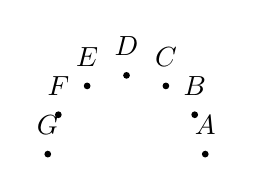
\begin{tikzpicture}
        \def \r {1} % Далее в документе \r будет заменяться на "1" (";" - не нужна)
        \coordinate (A) at (0:\r);
        \coordinate (B) at (30:\r);
        \coordinate (C) at (60:\r);
        \coordinate (D) at (90:\r);
        \coordinate (E) at (120:\r);
        \coordinate (F) at (150:\r);
        \coordinate (G) at (180:\r);
        \foreach \p in {A, ..., G} { % Поочерёдно записывать в \p буквы от A до G
            \draw [fill = black] (\p) circle(1pt);
            % \p LaTeX воспринимает, как обычную букву, но
            % (\p) LaTeX воспринимает, как точку (!)
            
            \node [label = above:$\p$] at (\p) {}; % Подпись точек
            % label = above: <-- метка будет размещена выше узла (можно: label = above left:)
            % $\p$ <-- содержимое метки
            % (\p) <-- позиция, где будет размещён узел
            % {} <-- Содержимое узла (здесь оно отсутствует), фактически аналог label, но LaTeX может неудовлетворительно его отобразить, в отличие от label
        }
    \end{tikzpicture}
\end{document}